\chapter{Introduction}
\label{sec:intro}

\section{Motivation}
\label{sec:intro:mo}

%Why are we doing it? About 1 page.§

%	bpmn introduce
	Business processes are fundamental elements for companies and organizations. They aggregate all the tasks, activities, and timelines involved in companies' workflow whose aim is to provide business services or to create value \cite{literature_review_2}. Business Process Modeling Notation, also known as BPMN, is a modeling language describing such workflows by using graphical notations and thus provides an easily understandable overview of the operations performed in the organization for all business users \cite{literature_review_1}. 
	
	Due to the importance of Business processes, leveraging the BPMN techniques can positively affect an organization's performance. Organizations can flexibly adapt to constantly changing business conditions through business process management by providing processes standardization, improvement and quick execution of the activities \cite{t2m_5}. However, not everyone is familiar with the BPMN designing techniques. Consequently, managers, along with other process participants prefer using natural language to define business processes. As a result, organizations usually have a large amount of information stored as text documents \cite{literature_review_2}. There is a need to transform these text documents into BPMN models. However process modeling is a complex task, it is often time-consuming, and experts with professional knowledge are required. According to \cite{t2m_5}, process modeling requires 60\% of the time within a business process management project. Adopting the approach that identifies and extracts process models can minimize the time and effort of the process modeling. \cite{literature_review_3} also suggests that  BPMN leads to process improvements, resulting in process cost reduction, quality increment, and higher revenue production. 
	%todo: if there is a need to expand the details of difficulties of process modeling, then refer to literature_review_2 
	
%	nlp introduce
	Over the past years, the development of AI techniques brought solutions to many technical difficulties. Natural Language Processing (NLP), as one of the AI's branches, could possibly address the problem of the difficulties in process modeling. Natural Language Processing is an interdisciplinary discipline focusing on the study of algorithms that enable the computer to understand and process the human language\cite{t2m_3}. During the understanding and processing of the natural language text, NLP performs three types of analysis: Firstly, morphological analysis is performed, which analyze the structure of words. The syntactic analysis then explores the grammar relationship between words in sentences, deciding which grammar category the word belongs to. Finally, semantic analysis is executed, which leverages the afore analyses to define the meaning of the text based on the knowledge of sentence structure and the relationship between words \cite{literature_review_2}. 
%if there is a need to expand the details of NLP analysis, then refer to literature_review_2 introduction part
	
%	why should nlp be used to generate the bpmn
	The unique features of the NLP technique make it very suitable for exploiting information from the text documents that record the firm's business process and then analyzing the data to generate the process models automatically. This paper serves as a proposal to suggest using NLP to extract the information from text written in nature language and automatically generate the corresponding business model.

\section{Research Questions}
\label{sec:intro:rq}

%At least 3 questions. They should not be answerable yes/no. Questions should be questions (1 sentence). But you are allowed to explain them in more detail. In the explanation also tell how you plan to prove that your potential future solution is good.
%
%About 1 page.

	The main research question (\textbf{RQ}) is formulated as: "\textit{How can business process models be automatically generated from textual descriptions using Natural language processing techniques?}". To better answer the main research question, three embedded aspects can be revealed: \textbf{RQ1}: "\textit{Which NLP methods can be used to extract information?}"; \textbf{RQ2}: "\textit{How can the extracted information be analyzed and composed to generate business process models?}" and finally \textbf{RQ3}: "\textit{How can the Large Language Models assist to improve the performance and the accuracy of the generated business process models}"

	
	Currently, there exist various tools, libraries, and dependencies for NLP. Therefore, the first research question \textbf{RQ1} tries to figure out which methods are the most suitable ones to use to extract information from textual descriptions. Currently, there exist several Natural language processing tools in academia and industry, and this work wants to explore their strengths and limitations. The work also aims to use the most suitable state-of-art-technique to perform the information extraction from the natural language text documents. 
	In the next step, \textbf{RQ2} explores how can the information in the text descriptions be analyzed and extracted and then be built into the business process model. The activities recognition here is an essential but challenging task here because the identified business activities and actors serve as a basis for the BPMN generation. To address this problem, the work aims to discover the typical structure of the business activities' textual representations in natural language documents by exploring the syntactical and grammatical relationships of the words. Furthermore, reconstructing the extracted business information is also challenging. The work will focus on identifying the conditional and sequential relationships of the business activities to develop algorithms that can generate a business process model with high accuracy.
	In light of the recent success of the Large Language Models (LLM) in natural language processing, they show great potential in semantic understanding and generating natural language text. A famous example is the \textit{ChatGPT} from the \textit{OpenAI}, where the \textit{ChatGPT} can help humans perform various tasks from article generation to code interpretation. Therefore, the last research question intends to determine whether Large Language Models can assist with the process model generation. \textbf{RQ3} tries to leverage the LLM to perform more through semantic analysis to facilitate and examine the generated BPMN diagram. A benchmarking will be performed to see what improvements is made.

	
	
	%	According to \cite{t2m_1}, the redundant information in the textual description input, such as examples, allows the human reader to understand the process better but will limit the performance of the BPMN generation. 
	
	
	%	The last research question \textbf{RQ3} tries to compare different complexity levels of the natural language documents. This research question aims to discover the adaptability of the proposed approach. The work will reveal the performance of our approach given natural language documents with different complexity levels, e.g., usual textual process descriptions, company policies, legal regulatory documents, and so on. Since such regulatory documents with higher complexity levels are always formulated in a more complex manner. The work should determine whether the explored extraction strategies still apply to such documents and whether the recognition accuracy drops. 


\section{Contribution}
\label{sec:intro:con}

%What will/have I do/done that nobody else has done before. About 1/2 page.

This work developed a tool that takes textual description as input and automatically generates a BPMN as output. The algorithms used in this work are mainly based on \cite{t2m_1}, which is considered to be the current state-of-art technique. Yet the work still sees room for improvement, and as a result, many modifications are made in order to improve the algorithms' performance and accuracy so that the generated BPMN models will be more accurate and logical as well as have a better visual effect. This work used \textit{Spacy} together with several open-sourced libraries, which are more up-to-date technologies compared to \cite{t2m_1}. As a result, such technologies could potentially lead to a better interpretation of generating BPMN models. Besides providing a BPMN diagram as output, the work also provides a formatted text output that can be used to render the BPMN diagram. By doing so, our tool provides great extensibility and offers users a simple way to improve the BPMN models and alter the generated output according to users' needs. The user can now generate and model the BPMN diagram with considerable time-saving with the help of our tool. Lastly, the work also explores the possibility of using Large Language Models such as \textit{GPT-4} in assisting BPMN model generation. The work leverages the LLM's ability to perform semantic analysis to improve the generated outcome and discover the strengths and weaknesses of BPMN model generation using LLM. The work also provides a suggestion on how to give the LLM the proper prompt to achieve a better result.

\section{Methodology}
\label{sec:intro:meth}

%Design Science in Information System (Hevner). How are we doing research?
%
%(1) Summary what design science is (it uses stakeholders, artefacts, steps, ...). (2) What are the stakeholders, artefacts, steps for MY case.

%About 1.5 pages.

Design science is a paradigm of real-world problem-solving by creating innovative artifacts. Therefore, Design science research tightly connected the IT artifact with the application domain. Furthermore, the need and desire to improve the current environment and methods motivate Design science research and thus requires innovative artifacts to address such problems \cite{DSM_1}. The work adopted the research methodology of \cite{DSM_2} here and followed the research process model given in their work.

\subsection{Problem centered approach}
Although some work in the current field was done, this work aims to develop better tools to automatically extract the business process model for the broad audience of end users, i.e., users within a business organization with little knowledge about business process modeling or underlying technologies. Such motivation provides us with an opportunity to work on creating the tool mentioned above. This problem-centered approach leads us to the first step of the research process, according to \cite{DSM_2}.

\subsection{Problem Identification And Motivation}
Current automated approaches that can create business process-visualizations from text are far from perfect, and there is significant room for improvement.

%Currently the automated approaches exists that can create business process visualizations from text in sufficient quality and generalizability

%Modeling business processes requires experts with relevant knowledge and can be exhausting and time-consuming. Thus, small companies usually cannot afford such experts and business managers usually prefer to describe processes using natural language. As a result, an organization usually process a large amount of text documents  \cite{literature_review_2}. However, the business process provides an intuitional overview of the business process and can potentially increase a company's productivity.

\subsection{Objectives of a solution}
Our objective is to create an easy-to-use tool that uses the Nature Language Processing technology to automatically extract information from organizations' texual documents and generate business process models.

\subsection{Design \& development}
The development of the new artifact adopted the critical success chain (CSC) method, which uses literature to support and consolidate the conceptual basis of the artifact designing \cite{DSM_2}. This work addressed the issues and the needs identified earlier, such as how to find a proper tool to extract information from texual documents or how to process such information to generate a BPMN model. The work conducted a literature review and used the helpful information from the selected papers to combine their ideas and develop our own artifact. The intended artifact is to develop a prototype that leverages the NLP technique to automatically extract business process models from texual documents.

\subsection{Demonstration}
In the demonstration activity, The work want to illustrate how can one use the proposed new artifact to solve instances of problem \cite{DSM_3}. The work will use the proposed artifact to convert the textual input into business process models where the users can quickly generate the BPMN models even though they have no knowledge of process modeling. We will run simulations to support our approach and to prove that our approach can minimize the workload of business process modeling.

\begin{figure}[h]
    \centering
    \caption{Design Science Research Process}
    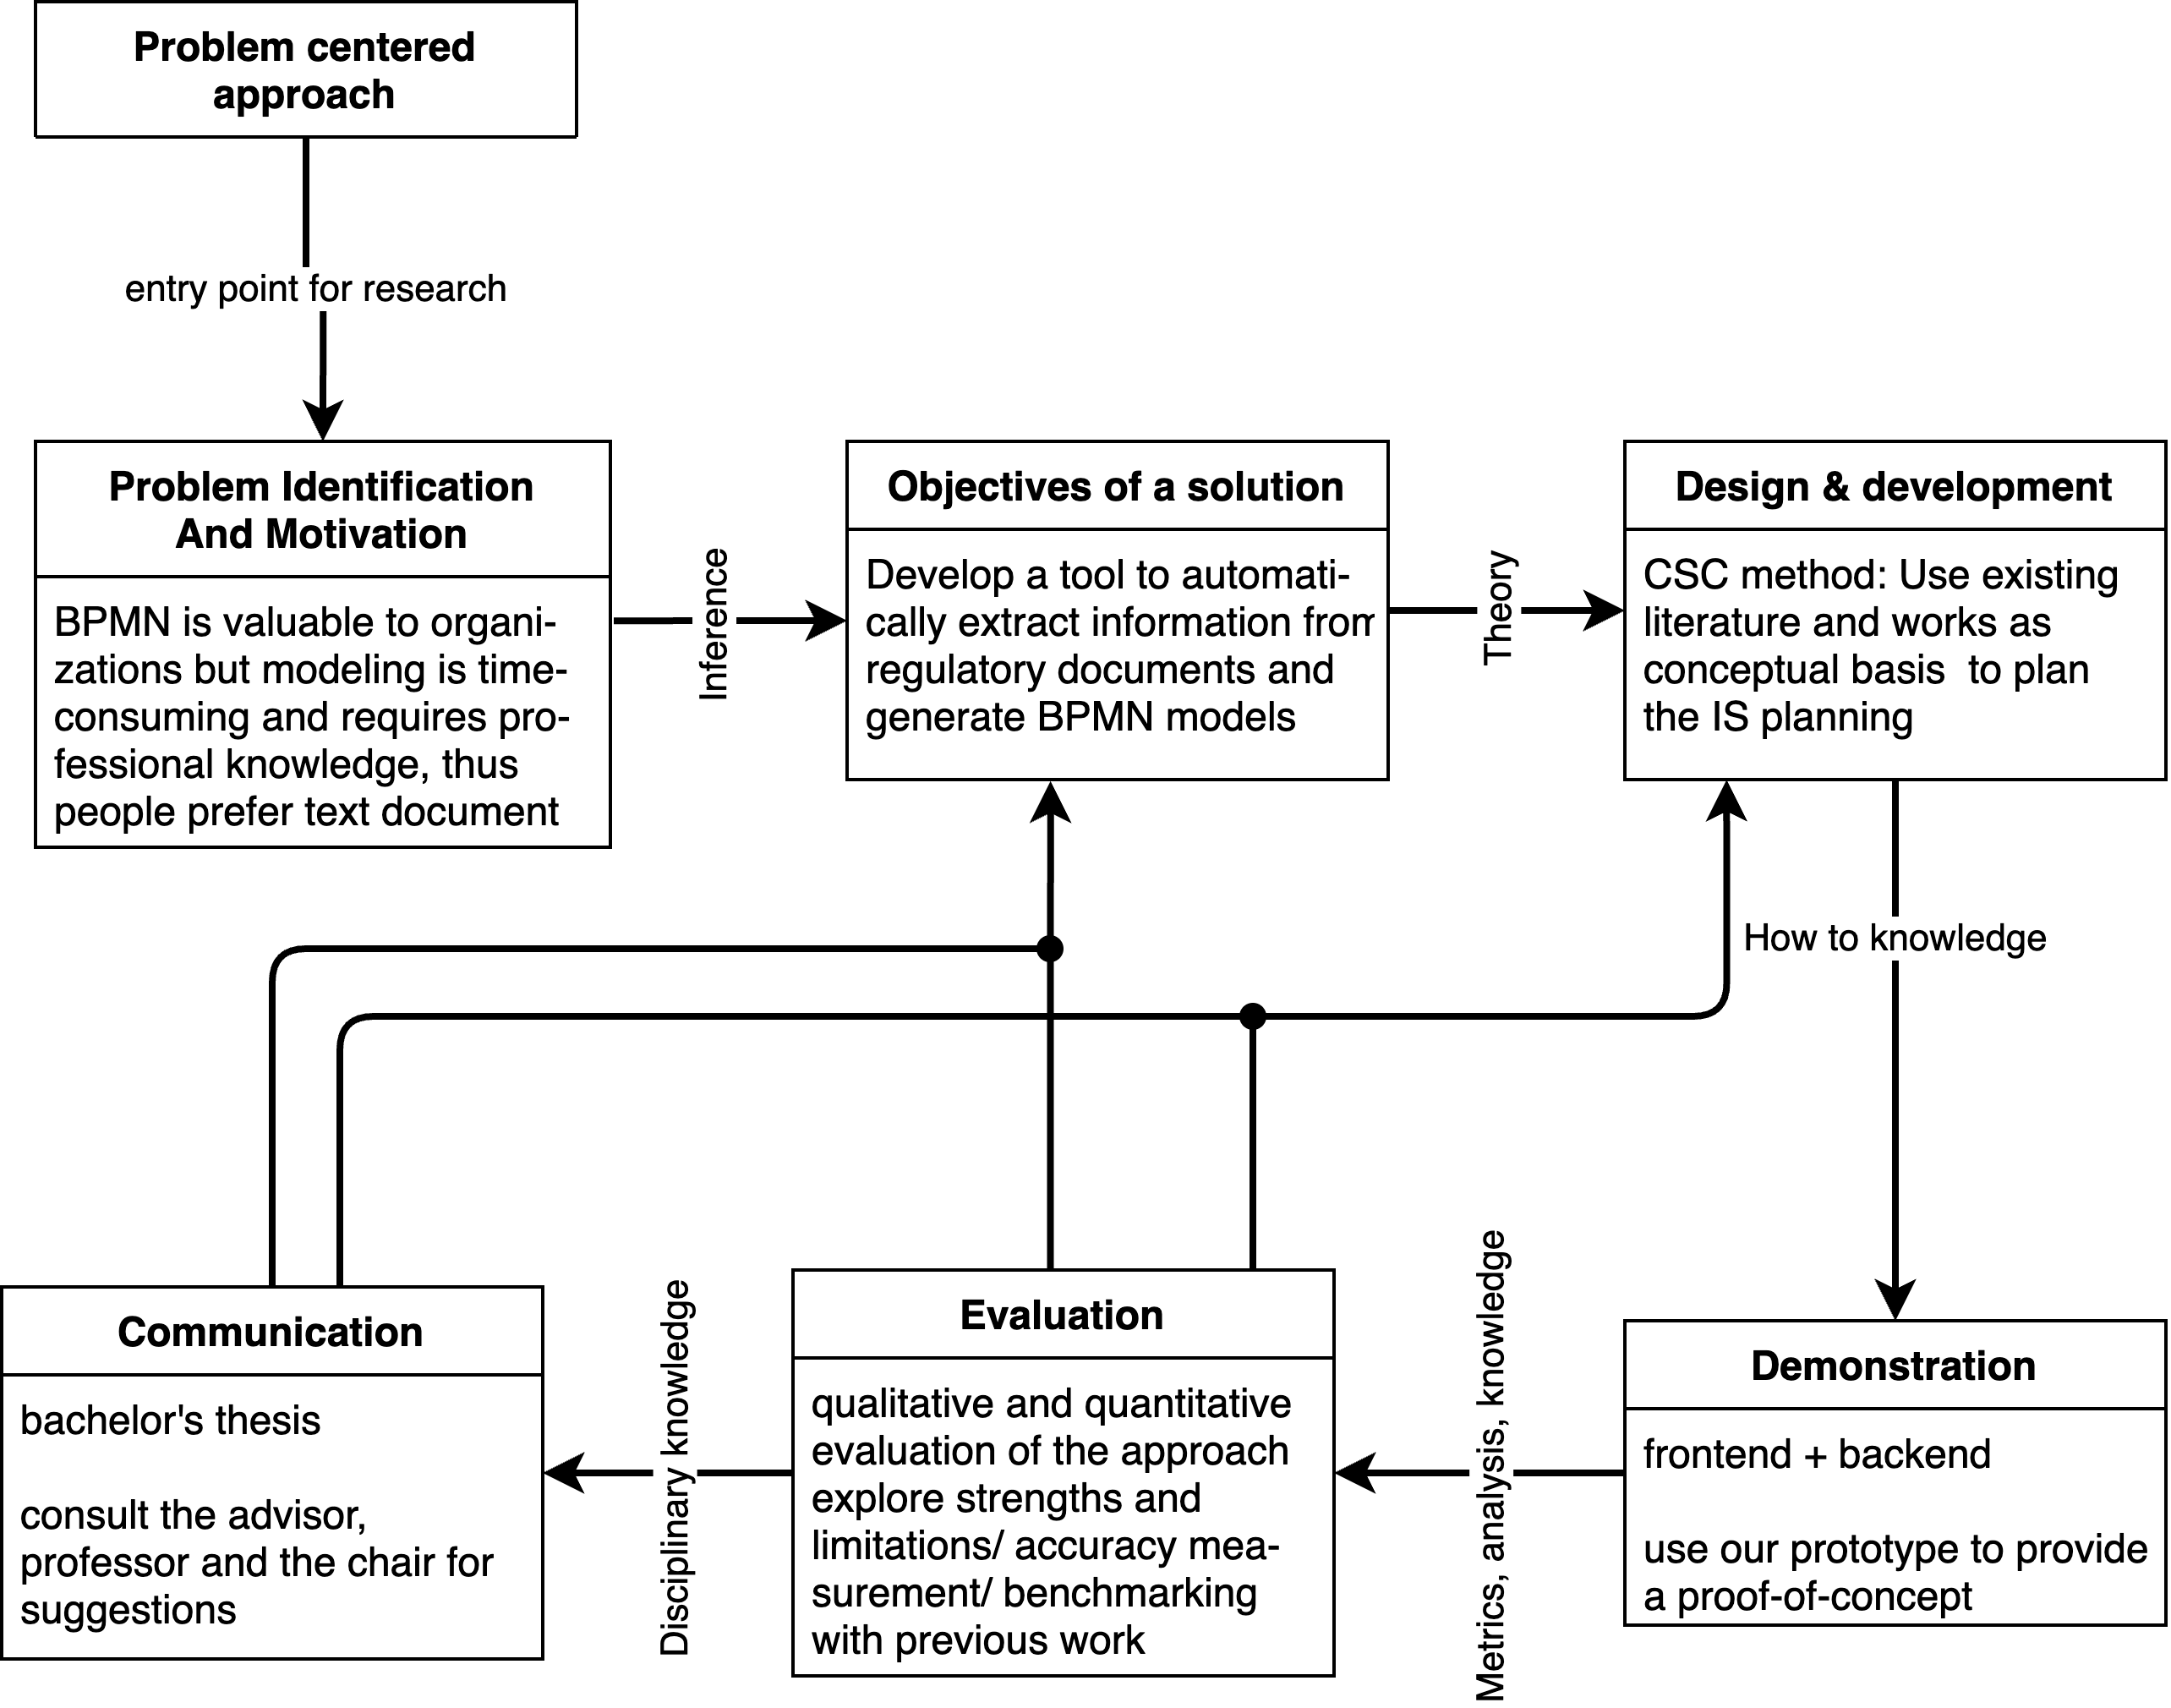
\includegraphics[width=0.9\textwidth]{tum-resources/images/DSM.png}
    \floatfoot{Overview of the research and artifact design steps for research methodology}
\end{figure}

\section{Evaluation}
\label{sec:intro:ev}
%How will I evaluate that my proposal is good. This ties into the research questions. About 1 page.

Evaluation is an essential aspect of artifact construction. It allows us to analyze the quality of the proposed artifact and based on which we can decide whether further modification and improvement should be made. The general goal of evaluation is whether the proposed approach satisfies the need of auto-generating BPMN models from textaul documents in actual practice and how well the proposed approach performs compared to previous works. The evaluation can be divided into to part: qualitative and quantitative evaluation.

In the quantitive evaluation, the work wants to compare how well the automatically extracted BPMN models approximate the previous work \cite{t2m_1_main} and the models created manually. In order to perform such accuracy benchmarking, this work will, in the first step, collect text documents from various sources and the corresponding BPMN diagram to construct the gold standard. Then, the same documents will be used as input for our approach and let the program automatically generate BPMN models. In the next stop, this work will summarize the generated activities, gateways, and lanes as well as calculate the correctness of the sequence flow by using the \textit{Log-based ordering relations} introduced in \cite{eva_02}. The work will also leverage the \textit{PET dataset} introduced in \cite{pet_dataset} to explore the relationship between redundant information and the accuracy of the generated BPMN diagram.

In the qualitative evaluation, the work plans to explore the pros and cons of the proposed approach compared to the standing works. During this phase, the components of the generated BPMN diagram will be analyzed to find out their strengths and limitations in handling different kinds of text input. The work will first compare with Friedrich's work given in \cite{t2m_1_main}, which is considered state-of-the-art, to see what new properties are introduced and what improvements are made to BPMN auto-generation. Then, the generated BPMN diagram will be used to compare with the diagram modeled by human experts to exploit the disadvantages of our approach. Finally, the evaluation analyzes the results modified using the Large Language Model to explore the feasibility of leveraging LLM in business process management. 


\section{Structure}
\label{sec:intro:struct}
The work consists of the following part: In section \ref{sec:rel}, a systematic literature is performed, and the related works are identified. Through the literature review, the work presents the current research gap as well as the strengths and weaknesses of the state-of-art technique. Section \ref{sec:solution} presents the potential challenges in the automatic generating process diagram from textual descriptions and the designed approaches to overcome such challenges. In section \ref{sec:implementation}, the actual implementations of the designed solution are presented with a series of vital algorithms used in the work listed. The section \ref{sec:evaluation} performs a series of qualitative and quantitative evaluation steps to verify our solution's improvement. In section \ref{sec:discussion}, the work discussed the designed approach and the possible next step. Finally, the section \ref{sec:conclusion} concludes the whole work.


